% =============================================
% =============================================
% Document class: Beamer
\documentclass[ 10pt, xcolor = dvipsnames]{beamer}
% Packages: Beamer
\usepackage{ beamerthemesplit, lmodern}
\setbeamertemplate{frametitle continuation}{}
% Packages: LaTeX (Depth-1)
\usepackage[ linesnumbered, ruled, vlined]{algorithm2e}
\usepackage{ amsfonts, amsmath, amssymb, amsthm}
\usepackage{ color, colortbl}
\usepackage{ dsfont}
\usepackage{ float}
\usepackage{ hhline}
\usepackage{ graphicx}
\usepackage{ latexsym}
\usepackage{ mathtools, multicol, multirow}
\usepackage{ parskip, pbox, pifont}
\usepackage{ ragged2e}
\usepackage{ setspace, stmaryrd, subcaption}
\usepackage{ tabularx}
\usepackage{ wasysym}
% Packages: LaTeX (Depth-2)
\usepackage{ epstopdf}

% =============================================
% Themes, colors and styles
\hypersetup{ colorlinks, linkcolor =, urlcolor = blue, citecolor = blue}
\usetheme{Madrid}
\usecolortheme[named=Brown]{structure}
\useinnertheme{rectangles}
\beamertemplatenavigationsymbolsempty

% =============================================
% =============================================
% Macros: Language
\newcommand{\define}{\triangleq}
\newcommand{\done}{\hfill $\square$}
%\newcommand{\eqCIRC}{\stackrel{\circ}{=}}
%\newcommand{\eqSTAR}{\stackrel{*}{=}}
\renewcommand{\epsilon}{\varepsilon}
\newcommand{\eg}{\textit{e.g.,\;}}
\newcommand{\egc}{\textit{e.g.:\;}}
\newcommand{\Eg}{\textit{E.g.,\;}}
\newcommand{\Egc}{\textit{E.g.:\;}}
\newcommand{\ie}{\textit{i.e.,\;}}
\newcommand{\iec}{\textit{i.e.:\;}}
\newcommand{\Ie}{\textit{I.e.,\;}}
\newcommand{\Iec}{\textit{I.e.:\;}}
\newcommand{\QED}{\hfill $\blacksquare$}
\renewcommand{\tilde}[1]{\widetilde{#1}}
\newcommand{\tsup}[1]{\ensuremath{^{\text{#1}}}}
\newcommand{\tsub}[1]{\ensuremath{_{\text{#1}}}}
\renewcommand{\vec}[1]{{\boldsymbol{#1}}}

% Macros: Optimization & Probability
\DeclareMathOperator*{\argmax}{arg\,max}
\DeclareMathOperator*{\argmin}{arg\,min}
\newcommand{\Exp}{\mathbb{E}}
\newcommand{\Indicate}[1]{ \IndFun \, \{ \, #1 \, \} }
\renewcommand{\Pr}{\mathbb{P}}
\newcommand{\Normal}{\mathcal{N}}
\newcommand{\std}{\text{std}}
\newcommand{\var}{\text{var}}

% Macros: Sets
\newcommand{\Complex}{\mathbb{C}}
\renewcommand{\emptyset}{\varnothing}
\newcommand{\Nat}{\mathbb{N}}
\renewcommand{\Re}{\mathbb{R}}
\newcommand{\ReNN}{{\Re}_{\geq 0}}
\newcommand{\ReSP}{{\Re}_{> 0}}
\renewcommand{\subset}{\subseteq}
\renewcommand{\supset}{\supseteq}
\newcommand{\Z}{\mathbb{Z}}
\newcommand{\ZNN}{{\Z}_{\geq 0}}

% Macros: Spacing & Other Commands
\newcommand{\fullcut}{\vspace{-\baselineskip}}
\newcommand{\fullskip}{\vspace{\baselineskip}}
\newcommand{\halfcut}{\vspace{-0.5\baselineskip}}
\newcommand{\halfskip}{\vspace{0.5\baselineskip}}
\renewcommand{\figurename}{Figura}
\renewcommand{\tablename}{Tabla}

% =============================================
% =============================================
\title[Din\'amica: Cap\'itulo 11]{Din\'amica: \textbf{Cap\'itulo 11} }
\author[Luis Reyes]{Luis I. Reyes Castro}
\institute[ESPOL]{\normalsize Escuela Superior Polit\'ecnica del Litoral (ESPOL) \\ Guayaquil - Ecuador}
\date[]{}

\AtBeginSection[]
{
\begin{frame}
\frametitle{Contenido del Tema}
\tableofcontents[ currentsection, sectionstyle = show/shaded, subsectionstyle = show/show/hide]
\end{frame}
}
\AtBeginSubsection[]
{
\begin{frame}
\frametitle{Contenido del Tema}
\tableofcontents[ currentsection, currentsubsection, sectionstyle = show/shaded, subsectionstyle = show/shaded/hide]
\end{frame}
}

% =============================================
\begin{document}

% =============================================
\begin{frame}[noframenumbering]
\titlepage
\end{frame}
%\begin{frame}[noframenumbering]
%\frametitle{Contenido del Tema}
%\tableofcontents[ subsectionstyle = hide]
%\end{frame}

% =============================================
\begin{frame}[allowframebreaks]
\frametitle{\S 11.3: Determinaci\'on del Movimiento de una Part\'icula}

Separaci\'on de Variables (``Magia Negra''): 
\begin{itemize}
\item Supongamos que en un problema tenemos dos variables $a(t)$ y $b(t)$ que \linebreak est\'an relacionadas por una \textbf{ecuaci\'on diferencial separable}: 
\[
\frac{da}{db} \; = \; \overbrace{ \; f(a) \; }^{ \mathclap{ \text{funci\'on de $a$} } } \underbrace{ \; g(b) \; }_{ \mathclap{ \text{funci\'on de $b$} } }
\]
\item Entonces es posible hallar una relaci\'on (aunque no siempre una funci\'on) entre $a(t)$ y $b(t)$ si tratamos la derivada $da/db$ como una fracci\'on y re-escribimos la ecuaci\'on anterior de la siguiente manera: 
\[
\frac{1}{f(a)} \, da \; = \; g(b) \, db
\]
\item Para encontrar la relaci\'on simplemente integramos ambos lados de la ecuaci\'on anterior: 
\[
\int_{a_0}^{a(t)} \frac{1}{f(\alpha)} \, d\alpha
\; = \; \int_{b_0}^{b(t)} g(\beta) \, d\beta
\]
\halfcut
\begin{itemize}
\item El lado izquierdo se integra con respecto a la primera variable ($a$) desde su \linebreak valor inicial $a_0$ hasta su valor actual $a(t)$. 
\item El lado derecho se integra con respecto a la segunda variable ($b$) desde su \linebreak valor inicial $b_0$ hasta su valor actual $b(t)$. 
\end{itemize}
\halfskip
\item Una vez evaluada la \'ultima integral, obtenemos una relaci\'on entre las dos variables que no involucra derivadas, \ie el lado izquierdo es una funci\'on \linebreak de $a(t)$ mientras que el lado derecho es una funci\'on de $b(t)$. 
\item Luego, dependiendo de la forma de esta relaci\'on, es posible que se pueda escribir a la variable $a(t)$ como una funci\'on de la variable $b(t)$. 
\end{itemize}

\end{frame}

% =============================================
\begin{frame}[allowframebreaks]
\frametitle{\S 11.3: Determinaci\'on del Movimiento de una Part\'icula}

Tres Casos: 
\begin{enumerate}
\item La aceleraci\'on es una funci\'on del tiempo, \iec 
\[
a \; = \; f(t)
\]
\item La aceleraci\'on es una funci\'on de la posici\'on, \iec 
\[
a \; = \; f(x)
\]
\item La aceleraci\'on es una funci\'on de la velocidad, \iec 
\[
a \; = \; f(v)
\]
\end{enumerate}

\end{frame}

% =============================================
\begin{frame}[allowframebreaks]
\frametitle{\S 11.3: Determinaci\'on del Movimiento de una Part\'icula}

Caso 1: La Aceleraci\'on es una Funci\'on del Tiempo
\begin{itemize}
\item Se nos indica que $a(t) = f(t)$. 
\item Recordando que  
\[
a(\tau) \; = \; \frac{dv}{dt} \bigg|_{ t = \tau }
\]
llegamos a la ecuaci\'on diferencial separable: 
\[
\frac{dv}{dt} \; = \; f(t)
\]
\framebreak
\item Aplicando separaci\'on de variables obtenemos: 
\begin{align*}
dv \; = \; f(t) \, dt \qquad 
& \Longrightarrow \qquad
\int_{v_0}^{v(t)} d\nu \; = \; \int_{0}^t f(\tau) \, d\tau \\[2ex]
& \Longrightarrow \qquad
v(t) - v_0 \; = \; \int_{0}^t f(\tau) \, d\tau \\[2ex]
& \Longrightarrow \qquad
v(t) = \; v_0 + \int_{0}^t f(\tau) \, d\tau
\end{align*}
\framebreak
\item Similarmente, dado que 
\[
v(\tau) \; = \; \frac{dx}{dt} \bigg|_{ t = \tau }
\]
llegamos a la ecuaci\'on diferencial separable: 
\[
\frac{dx}{dt} \; = \; v(t)
\]
\item Aplicando separaci\'on de variables obtenemos: 
\begin{align*}
x(t) \; 
& = \; x_0 + \int_{0}^{t} v(\tau) \, d\tau \\[2ex]
& = \; x_0 + v_0 \, t 
+ \int_0^t \left( \; \int_0^{\tau} f(u) \, du \, \right) d\tau
\end{align*}
\end{itemize}

\end{frame}

% =============================================
\begin{frame}[allowframebreaks]
\frametitle{\S 11.3: Determinaci\'on del Movimiento de una Part\'icula}

Caso 2: La Aceleraci\'on es una Funci\'on de la Posici\'on
\begin{itemize}
\item Se nos indica que: 
\[
a(t) = f( \, x(t) \, )
\]
\item Recordamos que hab\'iamos demostrado que: 
\[
a(\tau) \; = \; v(\tau) \, \frac{dv}{dx}\bigg|_{ t = \tau }
\]
\item Igualando estas dos expresiones para la aceleraci\'on obtenemos: 
\[
v \, \frac{dv}{dx} \; = \; f(x)
\]
\framebreak
\item Reconocemos que tenemos una ecuaci\'on diferencial separable: 
\[
\frac{dv}{dx} \; = \; \left( \frac{1}{v} \right) \, f(x)
\]
\item Finalmente, integrando la ecuaci\'on anterior obtenemos: 
\begin{align*}
v \, dv \; = \; f(x) \, dx \quad 
& \Longrightarrow \quad 
\int_{v_0}^{v(t)} \nu \, d\nu \; = \; 
\int_{x_0}^{x(t)} f( \xi ) \, d\xi \\[2ex]
& \Longrightarrow \quad 
\frac{1}{2} v(t)^2 - \frac{1}{2} v_0^2 \; = \; 
\int_{x_0}^{x(t)} f( \xi ) \, d\xi \\[2ex]
& \Longrightarrow \quad 
v(t) \; = \; 
\sqrt{ v_0^2 + 2 \int_{x_0}^{x(t)} f( \xi ) \, d\xi }
\end{align*}

\end{itemize}

\end{frame}

% =============================================
\begin{frame}[allowframebreaks]
\frametitle{\S 11.3: Determinaci\'on del Movimiento de una Part\'icula}

Caso 3: La Aceleraci\'on es una Funci\'on de la Velocidad
\begin{itemize}
\item Se nos indica que: 
\[
a(t) = f( \, v(t) \, )
\]
\item Recordamos que hab\'iamos demostrado que: 
\[
a(\tau) \; = \; v(\tau) \, \frac{dv}{dx}\bigg|_{ t = \tau }
\]
\item Igualando estas dos expresiones para la aceleraci\'on obtenemos: 
\[
v \, \frac{dv}{dx} \; = \; f(v)
\]
\framebreak
\item Reconocemos que tenemos una ecuaci\'on diferencial separable: 
\[
\frac{dv}{dx} \; = \; \left( \frac{1}{v} \right) \, f(v)
\]
\item Finalmente, integrando la ecuaci\'on anterior obtenemos: 
\begin{align*}
\frac{v}{f(v)} \, dv \; = \; dx \quad 
& \Longrightarrow \quad 
\int_{v_0}^{v(t)} \frac{\nu}{f(\nu)} \, d\nu \; = \; 
\int_{x_0}^{x(t)} d\xi \\[2ex]
& \Longrightarrow \quad 
\int_{v_0}^{v(t)} \frac{\nu}{f(\nu)} \, d\nu \; = \; 
x(t) - x_0 \\[2ex]
& \Longrightarrow \quad 
x(t) \; = \; x_0 + 
\int_{v_0}^{v(t)} \frac{\nu}{f(\nu)} \, d\nu
\end{align*}
\end{itemize}

\end{frame}

% =============================================
\begin{frame}[allowframebreaks]
\frametitle{Tarea 01}

Resuelva los problemas del texto gu\'ia (P\'ag. 613): 
\begin{itemize}
\item Problemas 11.7 y 11.8
\item Problemas 11.13 y 11.14
\item Problemas 11.19 y 11.20
\item Problema 11.24
\item Problemas desde el 11.27 hasta el 11.30
\end{itemize}
Fecha de entrega: Martes 1 de Noviembre de 2016

\end{frame}

% =============================================
\begin{frame}[allowframebreaks]
\frametitle{\S 11.4: Movimiento Rectil\'ineo Uniforme}

\begin{itemize}
\item La aceleraci\'on es cero en todo momento, \iec 
\[
a(t) \; = \; 0
\]
\item Consecuentemente: 
\begin{itemize}
\item La velocidad es constante. En particular: 
\[
v(t) \; = \; v
\]
\item La posici\'on es una funci\'on lineal en el tiempo. En particular: 
\[
x(t) \; = \; x_0 + v \, t
\]
\end{itemize}
\end{itemize}

\end{frame}

% =============================================
\begin{frame}[allowframebreaks]
\frametitle{\S 11.5: Movimiento Rectil\'ineo Uniformement Acelerado}

\begin{itemize}
\item La aceleraci\'on es constante, \iec 
\[
a(t) \; = \; a
\]
\item Consecuentemente: 
\begin{itemize}
\item La velocidad es una funci\'on lineal en el tiempo. En particular: 
\[
v(t) \; = \; v_0 + a \, t
\]
\item La posici\'on es una funci\'on cuadr\'atica en el tiempo. En particular: 
\[
x(t) \; = \; x_0 + v_0 \, t + \frac{1}{2} \, a \, t^2
\]
\end{itemize}
\end{itemize}

\end{frame}

% =============================================
\begin{frame}[allowframebreaks]
\frametitle{\S 11.6: Movimiento de Varias Part\'iculas}

Movimiento Relativo de Dos Part\'iculas: 
\begin{itemize}
\item Consideremos dos part\'iculas, denotadas $A$ y $B$. 
\begin{itemize}
\item La part\'icula $A$ tiene posici\'on $x_A$, velocidad $v_A$ y aceleraci\'on $a_A$. 
\item La part\'icula $B$ tiene posici\'on $x_B$, velocidad $v_B$ y aceleraci\'on $a_B$. 
\end{itemize}
\item Definimos la posici\'on relativa de la part\'icula $B$ con respecto a la part\'icula $A$, denotada $x_{B/A}$, de tal manera que: 
\[
x_{B/A} \; = \; x_B - x_A \qquad \Longleftrightarrow \qquad
x_B \; = \; x_A + x_{B/A}
\]
\item Similarmente, definimos la velocidad relativa de la part\'icula $B$ con respecto \linebreak a la part\'icula $A$, denotada $v_{B/A}$, de tal manera que: 
\[
v_{B/A} \; = \; v_B - v_A \qquad \Longleftrightarrow \qquad
v_B \; = \; v_A + v_{B/A}
\]
\item Adicionalmente, definimos la aceleraci\'on relativa de la part\'icula $B$ con respecto a la part\'icula $A$, denotada $a_{B/A}$, de tal manera que: 
\[
a_{B/A} \; = \; a_B - a_A \qquad \Longleftrightarrow \qquad
a_B \; = \; a_A + a_{B/A}
\]
\end{itemize}
\fullskip

Movimiento Dependiente (Problemas con Poleas): 
\begin{itemize}
\item El truco es primero escribir la longitud de la cuerda en funci\'on de las posiciones de las part\'iculas de inter\'es. 
\item Luego diferenciamos la expresi\'on para la longitud de la cuerda con respecto \linebreak al tiempo para encontrar una relaci\'on entre las velocidades de las part\'iculas de inter\'es. 
\item Finalmente diferenciamos la relaci\'on anterior con respecto al tiempo para encontrar una relaci\'on entre las aceleraciones de las part\'iculas de inter\'es. 
\end{itemize}

\end{frame}

% =============================================
\begin{frame}[allowframebreaks]
\frametitle{\S 11.6: Movimiento de Varias Part\'iculas}

\textbf{Ejemplo:}
\halfskip
\begin{columns}
\column{0.45\textwidth}
\begin{figure}
\centering
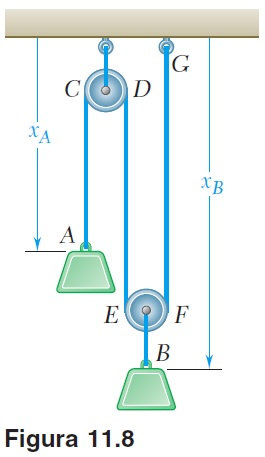
\includegraphics[ width = 0.5\columnwidth]{fig_11-8.jpg}
\end{figure}
\column{0.45\textwidth}
Si denotamos a la longitud de la cuerda como $\ell$ entonces: 
\[
\ell \; = \; x_A(t) + 2 \, x_B(t)
\]
Diferenciando la expresi\'on anterior obtenemos: 
\[
0 \; = \; v_A(t) + 2 \, v_B(t)
\]
Diferenciando la expresi\'on anterior obtenemos: 
\[
0 \; = \; a_A(t) + 2 \, a_B(t)
\]
\end{columns}

\end{frame}

% =============================================
\begin{frame}[allowframebreaks]
\frametitle{\S 11.6: Movimiento de Varias Part\'iculas}

\textbf{Ejemplo:}
\halfskip
\begin{columns}
\column{0.45\textwidth}
\begin{figure}
\centering
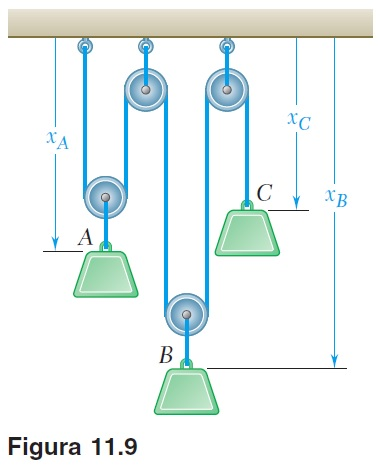
\includegraphics[ width = 0.7\columnwidth]{fig_11-9.jpg}
\end{figure}
\column{0.45\textwidth}
Si denotamos a la longitud de la cuerda como $\ell$ entonces: 
\[
\ell \; = \; 2 \, x_A(t) + 2 \, x_B(t) + x_C(t)
\]
Diferenciando la expresi\'on anterior obtenemos: 
\[
0 \; = \; 2 \, v_A(t) + 2 \, v_B(t) + v_C(t)
\]
Diferenciando la expresi\'on anterior obtenemos: 
\[
0 \; = \; 2 \, a_A(t) + 2 \, a_B(t) + a_C(t)
\]
\end{columns}

\end{frame}

% =============================================
\begin{frame}[allowframebreaks]
\frametitle{\S 11.6: Movimiento de Varias Part\'iculas}

\textbf{Ejercicio:} Problemas 11.47, 11.48, 11.49, 11.50. 
\halfskip
\begin{columns}
\column{0.45\textwidth}
\begin{figure}
\centering
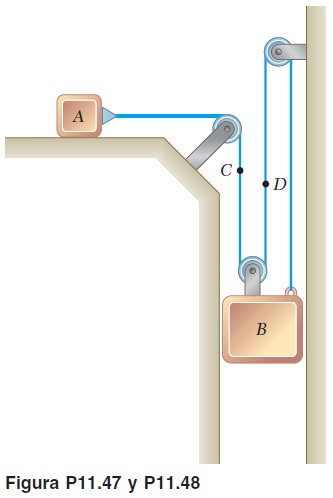
\includegraphics[ width = 0.8\columnwidth]{fig_P11-47_P11-48.jpg}
\end{figure}
\column{0.45\textwidth}
\begin{figure}
\centering
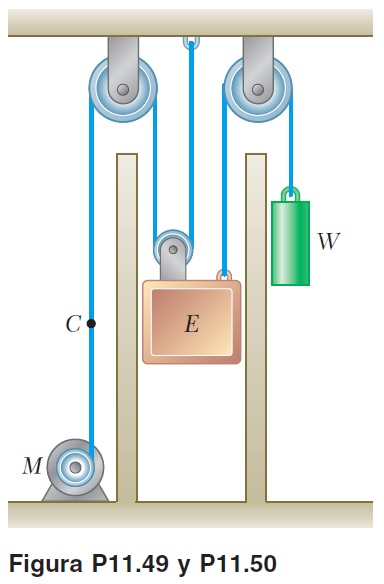
\includegraphics[ width = 0.6\columnwidth]{fig_P11-49_P11-50.jpg}
\end{figure}
\end{columns}

\end{frame}

% =============================================
\begin{frame}[allowframebreaks]
\frametitle{\S 11.6: Movimiento de Varias Part\'iculas}

\textbf{Ejercicio:} Problemas 11.51, 11.52. 
\halfskip
\begin{figure}
\centering
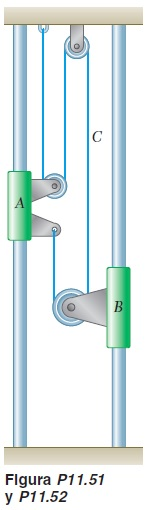
\includegraphics[ width = 0.16\columnwidth]{fig_P11-51_P11-52.jpg}
\end{figure}

\end{frame}

% =============================================
\begin{frame}[allowframebreaks]
\frametitle{\S 11.7-8: Soluci\'on Gr\'afica de Prob. de Mov. Rect.}

Recordamos que: 
\[
v(\tau) \; = \; \frac{dx}{dt} \bigg|_{ t = \tau } \qquad \qquad
a(\tau) \; = \; \frac{dv}{dt} \bigg|_{ t = \tau }
\]
\begin{figure}
\centering
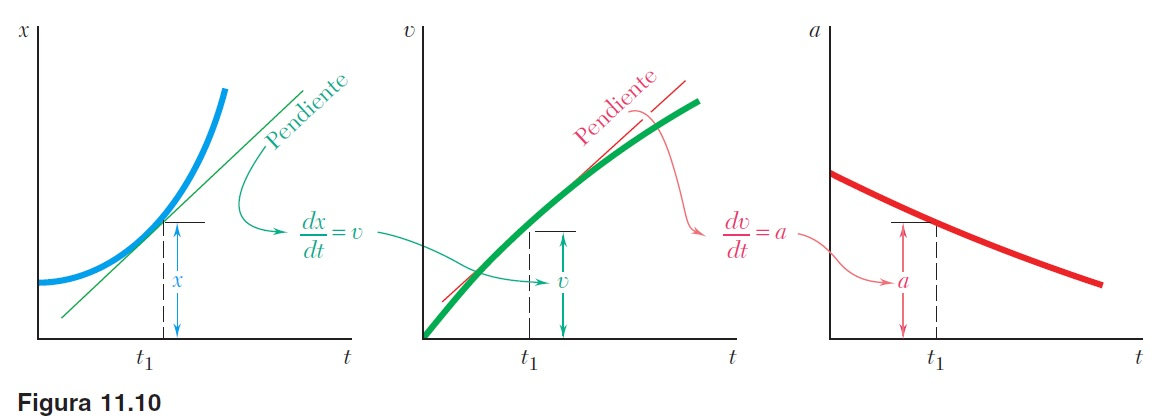
\includegraphics[ width = 0.6\textwidth]{fig_11-10.jpg}
\end{figure}

\framebreak

\begin{columns}
\column{0.4\textwidth}
Recordamos que: 
\begin{align*}
& v(t_2) - v(t_1) \; = \; \int_{t_1}^{t_2} a(\tau) \, d\tau \\[2ex]
& x(t_2) - x(t_1) \; = \; \int_{t_1}^{t_2} v(\tau) \, d\tau
\end{align*}
\column{0.5\textwidth}
\begin{figure}
\centering
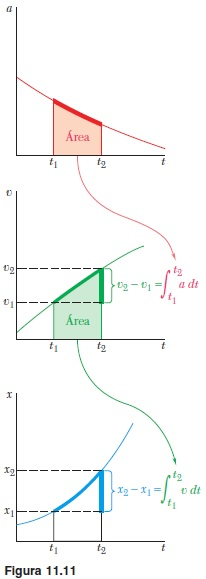
\includegraphics[ width = 0.4\columnwidth]{fig_11-11.jpg}
\end{figure}
\end{columns}

\end{frame}

% =============================================
%\begin{frame}[allowframebreaks]
%\frametitle{\S 11.7-8: Soluci\'on Gr\'afica de Prob. de Mov. Rect.}
%
%\textbf{Ejemplo: Problema Resuelto 11.6}
%
%Un vag\'on de transporte subterr\'aneo sale de la estaci\'on $A$; aumenta su rapidez a raz\'on de 4 ft/s\tsup{2} durante 6 s y despu\'es a raz\'on de 6 ft/s\tsup{2} hasta que llega a la rapidez de 48 ft/s. El vag\'on mantiene la misma rapidez hasta que se aproxima a la estaci\'on B; en ese momento se aplican los frenos, imparti\'endosele al vag\'on \linebreak una desaceleraci\'on constante y provocando que se detenga en 6 s. El tiempo de recorrido total desde $A$ hasta $B$ es de 40 s. Dibuje las curvas $a-t$, $v-t$ y \linebreak $x-t$ y determine la distancia entre las estaciones $A$ y $B$. 
%
%\begin{figure}
%\centering
%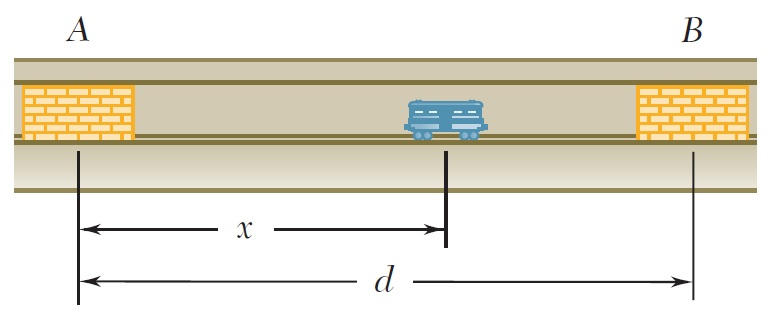
\includegraphics[ width = 0.4\textwidth]{fig_PR-11-6.jpg}
%\end{figure}
%
%\end{frame}

% =============================================
\begin{frame}[allowframebreaks]
\frametitle{Tarea 02}

Resuelva los siguientes problemas del texto gu\'ia: 
\begin{itemize}
\item Problemas 11.38, 11.46, 11.48, 11.50, 11.52, 11.55. 
\item Problemas 11.122, 11.124. 
\end{itemize}
Fecha de entrega: Martes 15 de Noviembre de 2016

\end{frame}

\end{document}
